\documentclass[12pt, letterpaper]{article}
\usepackage[utf8]{inputenc}
\usepackage{amsmath}
\usepackage{graphicx}
\graphicspath{ {.} }
\usepackage{wrapfig}
 
\title{Math 789 Assignment 4}
\author{Brendan Drachler}
\date{\today}

\begin{document}
\maketitle

\section*{Problem 3.1}

Starting from Eq. 3.1:

\begin{equation}
y(x)=\mathbf{w}_{0}+\mathbf{w}^{\top} x
\end{equation}

we will consider a point $\tilde{x}$ that lies on the decision boundary such that:

\begin{equation}
y(\tilde{x})=\mathbf{w}_{0}+\mathbf{w}^{\top} \tilde{x}
\end{equation}

Now, we will try to understand how we can characterize the distance between our point and the decision boundary.

\begin{equation}
y(x) - y(\tilde{x}) = \mathbf{w}^{\top} ( x - \tilde{x}) = 0
\end{equation}

This equation implies that $\mathbf{w}$ is orthogonal to the decision boundary containing point $\tilde{x}$.  Now, we can look at this geometrically as Bishop does in Figure 4.1 (in the newest edition of Pattern Recognition and Machine Learning). 

\begin{center}
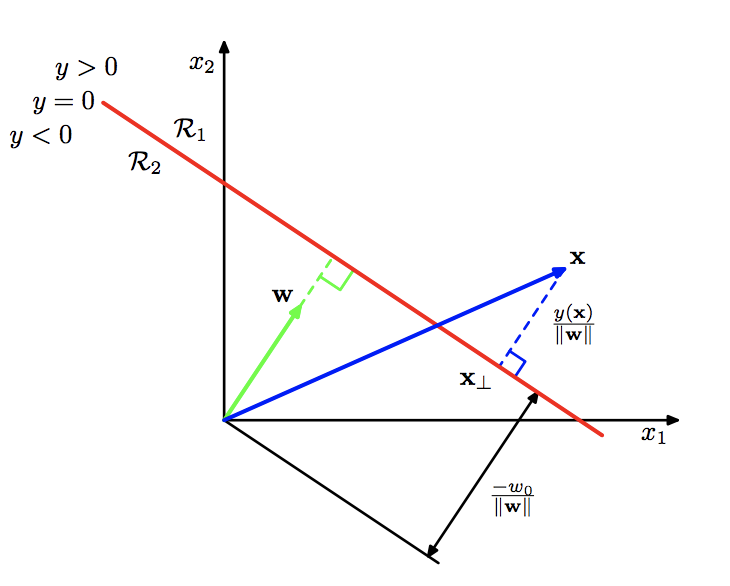
\includegraphics[scale=0.7]{problem_1_a.png}
\end{center}

We can now calculate the perpendicular distance, $L$, from the decision boundary to an arbitrary point $\mathbf{x}$. It is clear that the hypotenuse of our triangle is given by:

\begin{equation}
\mathbf{x}=\mathbf{x}_{\perp}+L \frac{\mathbf{w}}{\|\mathbf{w}\|}
\end{equation}

In this form, this equation doesn't help us much because we don't know what the form of $L$ is. But we do know that $y(\mathbf{x}_{\perp}) = 0$, because $\mathbf{x}_{\perp}$ is on the decision boundary. 

Therefore, we can write:

\begin{equation}
\mathbf{x}_{\perp} = \mathbf{x} - L \frac{\mathbf{w}}{\|\mathbf{w}\|}
\end{equation}

and 

\begin{equation}
y(\mathbf{x}_{\perp}) = \mathbf{w}_{0}+\mathbf{w}^{\top} \mathbf{x}_{\perp} = \mathbf{w}_{0}+\mathbf{w}^{\top} (\mathbf{x} - L \frac{\mathbf{w}}{\|\mathbf{w}\|}) = 0
\end{equation}

Multiplying out the last term and noting that $\mathbf{w}^{\top} \mathbf{w} = \|\mathbf{w}\|^2$ leads to:

\begin{equation}
\mathbf{w}_{0}+\mathbf{w}^{\top} \mathbf{x} - L \|\mathbf{w}\| = 0
\end{equation}
\begin{equation}
\mathbf{w}_{0}+\mathbf{w}^{\top} \mathbf{x} = L \|\mathbf{w}\|
\end{equation}

The left hand side of this equation is $y(\mathbf{x})$ which allows us to solve for $L$:

\begin{equation}
L = \frac{y(\mathbf{x})}{\|\mathbf{w}\|}
\end{equation}

\section*{Problem 3.2}

For this example, I will include Fig. 4.2 from the latest edition of Bishop's textbook for reference. 

In the case of $c = 3$, we will have 3 classes but only $(c-1) = (3-1) = 2$ linear discriminant functions. This is the example given on the left side of Bishop's figure. We know that: \newline
$\bullet \ \mathbf{x} \in C_{1}, y_{1}(\mathbf{x})>0$ \newline
$\bullet\  \mathbf{x} \in C_{2}, y_{2}(\mathbf{x})>0$ \newline  With this in mind, it is clear that the lower triangle has the property that $y_{1}(\mathbf{x})<0$ and $y_{3}(\mathbf{x})<0$. Therefore, that region is not ambiguous. The ambiguity stems from the upper region where  $y_{1}(\mathbf{x})>0$ and $y_{3}(\mathbf{x})>0$. It is not clear that values in that region should belong to any of the classes because there is no way to differentiate them from each other.

However, we can define our number of linear discriminant functions in a different way by declaring that when $c=3$, we have $c(c-1)/2 = 3(3-1)/2 = 3$ linear discriminant functions. We know that when: \newline

$\bullet \ (y_{12}(\mathbf{x})>0)$ and $(y_{13}(\mathbf{x})<0)$ then $(\mathbf{x} \in C_{1})$\newline 

$\bullet \ (y_{12}(\mathbf{x})<0)$ and $(y_{23}(\mathbf{x})<0)$ then $(\mathbf{x} \in C_{2})$\newline 

$\bullet \ (y_{13}(\mathbf{x})>0)$ and $(y_{23}(\mathbf{x})>0)$ then $(\mathbf{x} \in C_{3})$\newline

This leaves an ambiguous region when: \newline

$\bullet \ (y_{12}(\mathbf{x})<0)$ and $(y_{13}(\mathbf{x})<0)$ and $(y_{23}(\mathbf{x})>0)$ \newline


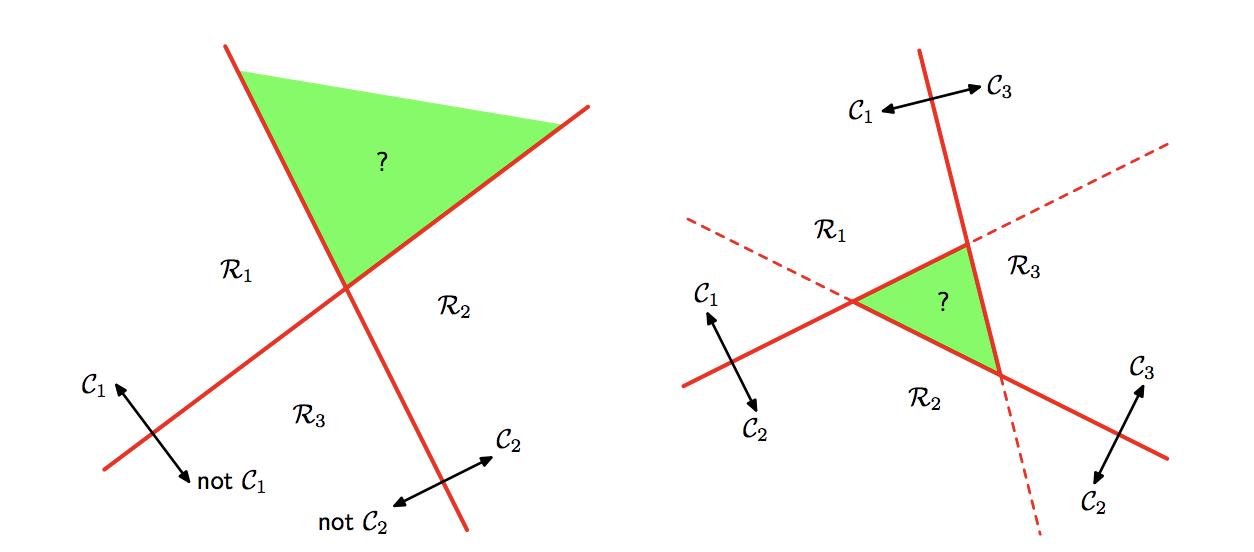
\includegraphics[scale=0.7]{problem_2_a.png}

\section*{Problem 3.6}

For this problem, I generated two normally distributed datasets with mean, $\mu_{1} = (10, 5)$ and $\mu_{2} = (5, 0)$ and a variance equal to the identity matrix. 

The gradient descent algorithm produces the following results. Instead of giving the lines after a set number of iterations, I chose to give them as a percentage of the total iterations. I chose this method of displaying the results because the total number of iterations is arbitrary based on what learning rate one chooses. In some instances, a given learning rate can cause there to be many thousands of iterations before convergence. 

\begin{center}
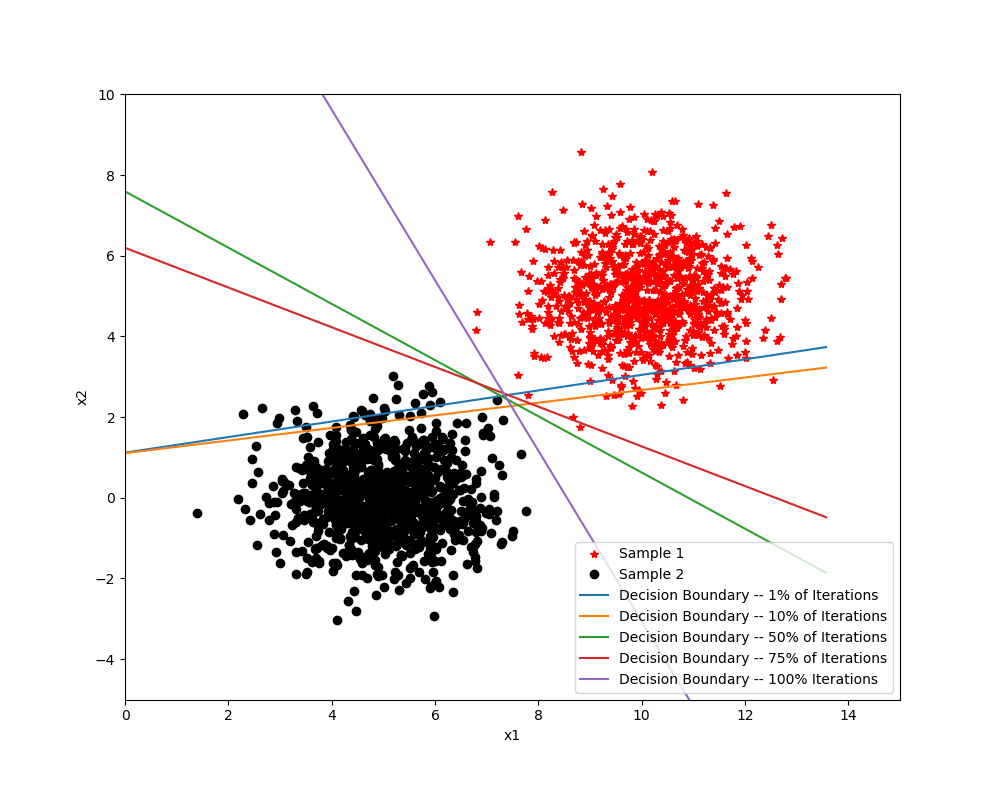
\includegraphics[scale=0.6]{problem_6_a.png}
\end{center}

The decision boundary is clearly performing very poorly for a low number of iterations but quickly improves. 

\section*{Problem 3.7}

Plug $y(x) = w x + w_0$ into Bishop Eq. 3.113:

\begin{equation}
E=3 \int_{0}^{3}\left[w^{2} x^{2}+\left(w_{0}-1\right)^{2}+2\left(w_{0}-1\right) w x\right] d x+\int_{4}^{5}\left[w^{2} x^{2}+\left(w_{0}+1\right)^{2}+2\left(w_{0}+1\right) w x\right] d x
\end{equation}

This trivially leads to:

\begin{equation}
E=\frac{142}{3} w^{2}+36 w w_{0}+10 w_{0}^{2}-18 w-16 w_{0}+10
\end{equation}

Now, we want to minimize the function with respect to $w$ and $w_0$. 

\begin{equation}
\frac{\partial E}{\partial w} = \frac{284}{3} w + 36 w_0 - 18 = 0
\end{equation}
\begin{equation}
\frac{\partial E}{\partial w_0} = 36 w + 20 w_0 - 16 = 0
\end{equation}

Solving these two equations for $w$ and $w_0$ leads to $w = -0.36161$ and $w_0 = 1.4509$. Thus, the linear discriminant function separating these two classes is $y(x) =  -0.36161 x + 1.4509$. Does this linear discriminant function work at $y(x) = 0$?

\begin{equation}
y(x) =  -0.36161 x + 1.4509 = 0
\end{equation}
\begin{equation}
x \approx 4.0123
\end{equation}

$x \approx 4.0123$ fails to separate the boundaries because it falls within class $C_2$. 

A single layer perceptron could separate the two classes because they are clearly linearly separable and the perceptron convergence theorem states that convergence will be reached in a finite number of steps. Though, the number of steps can still be substantial compared to least-squares. However, there is no guarantee that least-squares will converge on a boundary that linearly separates the two classes.

\section*{Problem 3.11}
Starting from Bishop Eq. 3.90:

\begin{equation}
\sum_{n=1}^{N}\left(\mathbf{w}^{\mathrm{T}} \mathbf{x}^{n}+w_{0}-t^{n}\right) \mathbf{x}^{n}=0
\end{equation}

Multiplying through by $\mathbf{x}^n$, utilizing Bishop Eq. 3.91, and considering that $t^n$ takes on the value $N/N1$ for class $C_1$ and $-N/N2$ for class $C_2$ we can simplify our expression to:

\begin{equation}
\sum_{n=1}^{N} \mathbf{x}_{\mathbf{n}} \mathbf{x}_{\mathbf{n}}^{T} \mathbf{w}-\mathbf{w}^{T} \mathbf{m} \cdot(N \mathbf{m})-\left(\sum_{n \in C_{1}} \frac{N}{N_{1}} \mathbf{x}_{\mathbf{n}}+\sum_{n \in C_{2}} \frac{-N}{N_{2}} \mathbf{x}_{\mathbf{n}}\right) = 0
\end{equation}

We can now use Bishop Eq. 3.98 to simplify further. 

\begin{equation}
\sum_{n=1}^{N} \mathbf{x}_{\mathbf{n}} \mathbf{x}_{\mathbf{n}}^{T} \mathbf{w}-N \mathbf{m m}^{T} \mathbf{w} = N\left(\mathbf{m}_{1}-\mathbf{m}_{2}\right)
\end{equation}

We now have the right hand side of Bishop Eq. 3.93. We need to work the left hand side further. 

\begin{equation}
LHS = w [\sum_{n=1}^{N} \mathbf{x}_{\mathbf{n}} \mathbf{x}_{\mathbf{n}}^{T}-N\left(\frac{N_{1}}{N} \mathbf{m}_{1}+\frac{N_{2}}{N} \mathbf{m}_{2}\right)^{2}]
\end{equation}

\begin{equation}
=w [\sum_{n=1}^{N} \mathbf{x}_{\mathbf{n}} \mathbf{x}_{\mathbf{n}}^{T}-\frac{N_{1}^{2}}{N}\left\|\mathbf{m}_{1}\right\|^{2}-\frac{N_{2}^{2}}{N}\left\|\mathbf{m}_{2}\right\|^{2}-2 \frac{N_{1} N_{2}}{N} \mathbf{m}_{1} \mathbf{m}_{2}^{T}]
\end{equation}

\begin{equation}
\begin{aligned}
&=w [\sum_{n=1}^{N} \mathbf{x}_{\mathbf{n}} \mathbf{x}_{\mathbf{n}}^{T}+\left(N_{1}-2 N_{1}\right)\left\|\mathbf{m}_{1}\right\|^{2}+\left(N_{2}-2 N_{2}\right)\left\|\mathbf{m}_{2}\right\|^{2}+\frac{N_{1} N_{2}}{N}\left\|\mathbf{m}_{1}-\mathbf{m}_{2}\right\|^{2} ]\\
&=w [ \sum_{n=1}^{N} \mathbf{x}_{\mathbf{n}} \mathbf{x}_{\mathbf{n}}^{T}+N_{1}\left\|\mathbf{m}_{\mathbf{1}}\right\|^{2}-2 \mathbf{m}_{\mathbf{1}} \sum_{n \in C_{1}} x_{n}^{T}+N_{2}\left\|\mathbf{m}_{\mathbf{2}}\right\|^{2}-2 \mathbf{m}_{\mathbf{2}} \sum_{n \in C_{2}} x_{n}^{T}+\frac{N_{1} N_{2}}{N} \mathbf{S}_{\mathbf{B}} ]\\
&=w [\sum_{n \in C_{1}} \mathbf{x}_{\mathbf{n}} \mathbf{x}_{\mathbf{n}}^{T}+N_{1}\left\|\mathbf{m}_{1}\right\|^{2}-2 \mathbf{m}_{1} \sum_{n \in C_{1}} x_{n}^{T} ]\\
&=w [\sum_{n \in C_{1}}\left(\mathbf{x}_{\mathbf{n}} \mathbf{x}_{\mathbf{n}}^{T}+\left\|\mathbf{m}_{\mathbf{1}}\right\|^{2}-2 \mathbf{m}_{\mathbf{1}} x_{n}^{T}\right)+\sum_{n \in C_{2}}\left(\mathbf{x}_{\mathbf{n}} \mathbf{x}_{\mathbf{n}}^{T}+\left\|\mathbf{m}_{\mathbf{2}}\right\|^{2}-2 \mathbf{m}_{\mathbf{2}} \mathbf{x}_{\mathbf{n}}^{T}\right)+\frac{N_{1} N_{2}}{N} \mathbf{S}_{\mathbf{B}} ]\\
&=w[\sum_{n \in C_{1}}\left\|\mathbf{x}_{\mathbf{n}}-\mathbf{m}_{\mathbf{1}}\right\|^{2}+\sum_{n \in C_{2}}\left\|\mathbf{x}_{\mathbf{n}}-\mathbf{m}_{\mathbf{2}}\right\|^{2}+\frac{N_{1} N_{2}}{N} \mathbf{S}_{\mathbf{B}}]\\
&=w[\mathbf{S}_{\mathbf{w}}+\frac{N_{1} N_{2}}{N} \mathbf{S}_{\mathbf{B}}]
\end{aligned}
\end{equation}

This validates Bishop Eq. 3.93. 

\begin{equation}
\begin{aligned}
LHS = RHS \\
w[\mathbf{S}_{\mathbf{w}}+\frac{N_{1} N_{2}}{N} \mathbf{S}_{\mathbf{B}}] = N\left(\mathbf{m}_{1}-\mathbf{m}_{2}\right)
\end{aligned}
\end{equation}

\section*{Problem 3.12}

Our goal is to utilize the following two equations:

\begin{equation}
\mathbf{m}_{k}=\frac{1}{N_{k}} \sum_{\mathbf{n} \in \mathcal{C}_{k}} \mathbf{x}^{n}
\end{equation}
\begin{equation}
\mathbf{S}_{T}=\sum_{n=1}^{N}\left(\mathbf{x}^{n}-\mathbf{m}\right)\left(\mathbf{x}^{n}-\mathbf{m}\right)^{\mathbf{T}}
\end{equation}

to prove that $\mathbf{S}_{T}$ can be decomposed into two independent components of the covariance matrix given by:

\begin{equation}
\mathbf{S}_{T} = \mathbf{S}_{W} + \mathbf{S}_{B}
\end{equation}

where  $\mathbf{S}_{W}$ and $ \mathbf{S}_{B}$ are given by:

\begin{equation}
\mathbf{S}_{B}=\sum_{k=1}^{c} N_{k}\left(\mathbf{m}_{k}-\mathbf{m}\right)\left(\mathbf{m}_{k}-\mathbf{m}\right)^{\mathbf{T}}
\end{equation}
\begin{equation}
\mathbf{S}_{W}=\sum_{k=1}^{c} \mathbf{S}_{k} =\sum_{k=1}^{c}(\mathbf{x}^{n}-\mathbf{m}_{k})(\mathbf{x}^{n}-\mathbf{m}_{k})^{\mathbf{T}}
\end{equation}

We will begin by expanding $\mathbf{S}_{T}$ as follows:

\begin{equation}
\mathbf{S}_{T}=\sum_{k=1}^{c} \sum_{n=1}^N\left(\mathbf{x}^n-\mathbf{m}_{k}+\mathbf{m}_{k}-\mathbf{m}\right)\left(\mathbf{x}^n-\mathbf{m}_{k}+\mathbf{m}_{k}-\mathbf{m}\right)^{\mathbf{T}}
\end{equation}

We can now expand the inside of the summation by grouping the first two terms and the last two terms of each member of the product.

\begin{multline}
\mathbf{S}_{T}=\sum_{k=1}^{c} \sum_{n=1}^N(\mathbf{x}^n -\mathbf{m}_{k})(\mathbf{x}^n -\mathbf{m}_{k})^{\mathbf{T}} + \sum_{k=1}^{c} \sum_{n=1}^N(\mathbf{m}_k -\mathbf{m})(\mathbf{m}_k -\mathbf{m})^{\mathbf{T}} \\
+ \sum_{k=1}^{c} \sum_{n=1}^{N}[(\mathbf{x}^{n}-\mathbf{m}_{k})({\mathbf{m}_{k}-\mathbf{m})^{\mathbf{T}}+(\mathbf{m}_{k}-\mathbf{m})(\mathbf{x}^{n}-\mathbf{m}_{k})^{\mathbf{T}}}] 
\end{multline}

Notice that the first term is $\mathbf{S}_{W}$ and the second term is 
$\mathbf{S}_{B}$. We still need to deal with the last two terms by utilizing the first equation in this section.

\begin{multline}
\mathbf{S}_{T}= \mathbf{S}_{W} + \mathbf{S}_{B}
+ \sum_{k=1}^{c} \sum_{n=1}^{N}[(\mathbf{x}^{n}-\mathbf{m}_{k})({\mathbf{m}_{k}-\mathbf{m})^{\mathbf{T}}+(\mathbf{m}_{k}-\mathbf{m})(\mathbf{x}^{n}-\mathbf{m}_{k})^{\mathbf{T}}}] 
\end{multline}

Let's focus on the following term that shows up in the left over pieces of the expression:

\begin{multline}
\sum_{n=1}^{N}(\mathbf{x}^{n}-\mathbf{m}_{k}) = N_k \mathbf{m}_k-\sum_{n=1}^{N}\mathbf{m}_{k} = N_k \mathbf{m}_k - N_k \mathbf{m}_k = 0 \\
\Downarrow \\
\sum_{k=1}^{c} \sum_{n=1}^{N}[(\mathbf{x}^{n}-\mathbf{m}_{k})({\mathbf{m}_{k}-\mathbf{m})^{\mathbf{T}}+(\mathbf{m}_{k}-\mathbf{m})(\mathbf{x}^{n}-\mathbf{m}_{k})^{\mathbf{T}}}]  = 0
\end{multline}

Therefore, $\mathbf{S}_{T}= \mathbf{S}_{W} + \mathbf{S}_{B}$. 



\end{document}